\chapter{Gamma Function}
\minitoc
This chapter discusses the gamma function, the log gamma function and the incomplete Gamma function. 

\section{Gamma Function}
The Gamma function is defined as the following integral
\[ \Gamma(x) = \int_0^\infty t^{x-1} e^{-t}dt\]
on $(-\infty, \infty)$ except 0 and negative integers. It is an extension of the factorial function for positive integers.
Here are some basic facts:
\begin{enumerate}
\item For positive integer n, $\Gamma(n) = (n-1)!$ with $0! = 1$.
\item For any real x in the domain, $\Gamma(x) = x\Gamma(x-1)$.
\item For any real x in the domain, 
\[\Gamma(1 - x)\Gamma(x) = \frac{\pi}{sin(\pi x)}\] 
This is called Euler's reflection and can be used to compute gamma function values for negative x if we know the values for positive x.
\item $\Gamma(x)$ is asymptotic to $\frac{1}{x}$ when $x \rightarrow 0$, and it asymptotic to $\Big(\frac{x}{e}\Big)^x \sqrt{\frac{2\pi}{x}}$  when $x \rightarrow \infty$ 
\end{enumerate} 
The graph of the gamma function is below. 
\begin{figure*}[htp]
\begin{center}
{
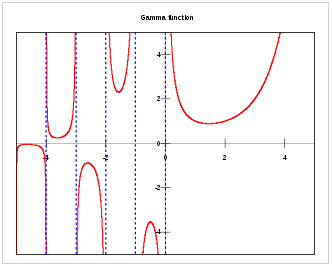
\includegraphics[bb=-90 0 400 250,width=1\textwidth] {chap3/gamma.png}
}
\end{center}
\caption{Gamma Function, from wiki}
\label{figure:gammafunction}
\end{figure*}

When x > 171.624, the gamma function value is too large to fit into a double and thus causes overflow. One way to get around this is to use log gamma function in the next section.

We tested several implementations:
\begin{itemize}
\item log gamma based implementation
\item The cephes lib implmentation
\item The Cody implementation
\item Lanzcos 15-term implementation
\item The implementation based on the reciprocal gamma function
\item The implementation based on Pugh's Thesis
\end{itemize}
Accuracy and Performance.

\section{Log Gamma Function}
The log gamma function is the log of the gamma function defined on the positive real axis. The graph of the gamma function is below. 
\begin{figure*}[htp]
\begin{center}
{
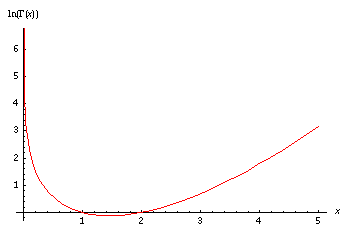
\includegraphics[bb=-90 0 300 200,width=1\textwidth] {chap3/loggamma.png}
}
\end{center}
\caption{Log Gamma Function, from MathWorld}
\label{figure:loggammafunction}
\end{figure*}

The implementation is translated from fdlibm53. However, since loggamma is zero when x = 1 and 2. The original implementation suffers from cancellation near these two points. One way to fix it is to use BigDecimal, though it suffers performance hit. 

Accuracy and Performance.

\section{Incomplete Gamma Function}
The gamma function is definted as a definite integral over a constant interval $(0, \infty)$. By changing the interval, we can define the incomplete gamma function. The upper incomplete gamma function is defined as the following integral
\[ \Gamma(a, x) = \int_x^\infty t^{a-1} e^{-t}dt\]
The lower incomplete gamma function is defined as
\[ \gamma(a, x) = \int_0^x t^{a-1} e^{-t}dt\]
and thus 
\[ \Gamma(a, x) + \gamma(a, x) = \Gamma(a) \]
Now scale $\Gamma(a, x)$ and $\gamma(a, x)$ by $\Gamma(a)$, we yield the normalized definitions:
\[ P(a, x) = \frac{\gamma(a, x)}{\Gamma(a)} = \frac{1}{\Gamma(a)}\int_0^x t^{a-1} e^{-t}dt\]
and 
\[ Q(a, x) = \frac{\Gamma(a, x)}{\Gamma(a)} = \frac{1}{\Gamma(a)}\int_x^\infty t^{a-1} e^{-t}dt\]
These functions are defined in the domain $a > 0$ and $x >= 0$. Here are some basic facts for $P(a, x)$:
\begin{enumerate}
\item the range of the function is $[0, 1)$.
\item the function changes most rapidly around $x = a$.
\item the function is strictly increasing for x when a is fixed.
\item if $a > b$, then $P(a, x) < P(b, x)$ for all x.
\item $P(0, x) = 1 + \operatorname{Ei}(-x)$???
\item if $a \rightarrow \infty$, $P(a, x) \rightarrow 0$ for all x.???
\end{enumerate}
The graph for $P(a, x)$ is showing some of the above properties.
\begin{figure*}[htp]
\begin{center}
{
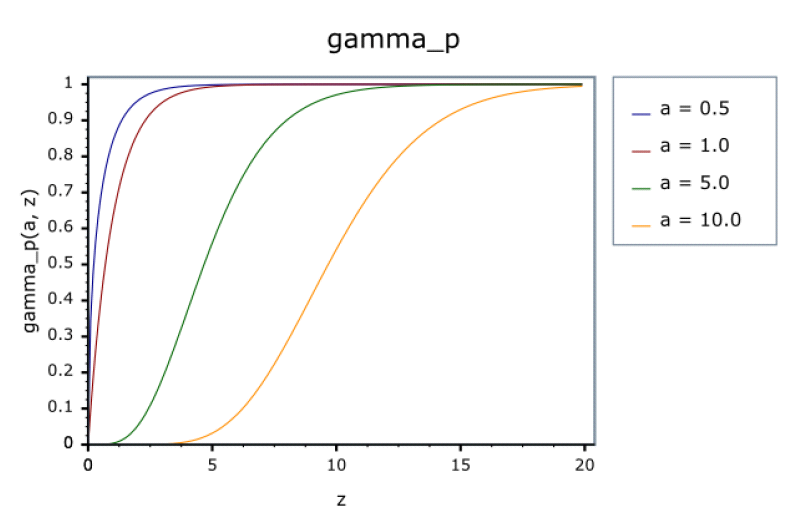
\includegraphics[bb=0 0 600 400,width=1\textwidth] {chap3/gammap.png}
}
\end{center}
\caption{Normalized Lower incomplete Gamma Function, from Boost}
\label{figure:gammapfunction}
\end{figure*}

Similarly, here are some basica facts for $Q(a, x)$:
\begin{enumerate}
\item the range of the function is $[0, 1)$.
\item the function changes most rapidly around $x = a$.
\item the function is strictly decreasing for x when a is fixed.
\item if $a > b$, then $Q(a, x) > Q(b, x)$ for all x.
\item $Q(0, x) = - \operatorname{Ei}(-x)$???
\item if $a \rightarrow \infty$, $P(a, x) \rightarrow 0$ for all x.???
\end{enumerate}
The graph for $Q(a, x)$ shows some of the above properties.
\begin{figure*}[htp]
\begin{center}
{
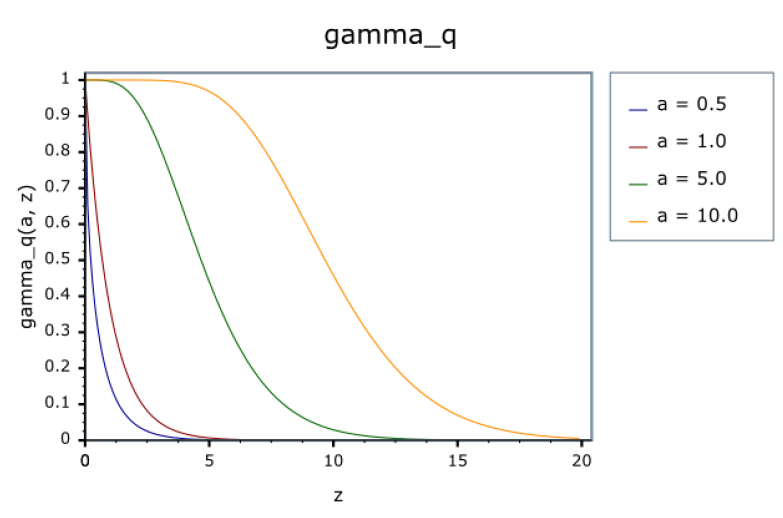
\includegraphics[bb=0 0 600 400,width=1\textwidth] {chap3/gammaq.png}
}
\end{center}
\caption{Normalized Upper incomplete Gamma Function, from Boost}
\label{figure:gammaqfunction}
\end{figure*}


\section{Reference}

Java implementations:
\begin{itemize}
\item JLapack: http://www.netlib.org/lapack/
\item Colt implementation:
\item Jsci implementation:
\item ojAlgo
\item Jama
\item Jampack
\item UJMP: http://www.ujmp.org/
\end{itemize}

Other implementations:
\begin{itemize}
\item Aglib: for C++, .net
\item newmat: a good C++ implementation
\item BLAS: http://www.netlib.org/blas/
\item BOOST: http://www.boost.org/ 
\item PLapack C implementation: http://www.cs.utexas.edu/~plapack/
\end{itemize}

BLAS

\begin{thebibliography}{99}

% >>>>>>>>> Book examples <<<<<<<<<
\bibitem{CarpenterBOOK} Carpenter, R.H.S., {\textit Movements of the Eyes},
 2nd Edition, Pion Publishing, 1988.

\bibitem{FranklinBOOK} Franklin, G.F., Powel, J.D., Workman, M.L.,
{\textit Digital Control of Dynamic Systems}, Second Edition,
Addison-Wesley, 1990.

% >>>>>>>>> Conference Proceedings Example <<<<<<<<<
\bibitem{OhICRA1998} Oh, P.Y., Allen, P.K., ``Design a Partitioned
 Visual Feedback Controller,'' {\textit IEEE Int Conf Robotics
 \& Automation}, Leuven, Belgium, pp. 1360-1365 5/98

% >>>>>>>>> Journal Example <<<<<<<<<<<<<<<<<<<<<<<<
\bibitem{OhTRA2001} Oh, P.Y., Allen, P.K., ``Visual Servoing
 by Partitioning Degrees of Freedom,'' {\textit IEEE Trans on 
 Robotics \& Automation}, V17, N1, pp. 1-17, 2/01

\end{thebibliography}
